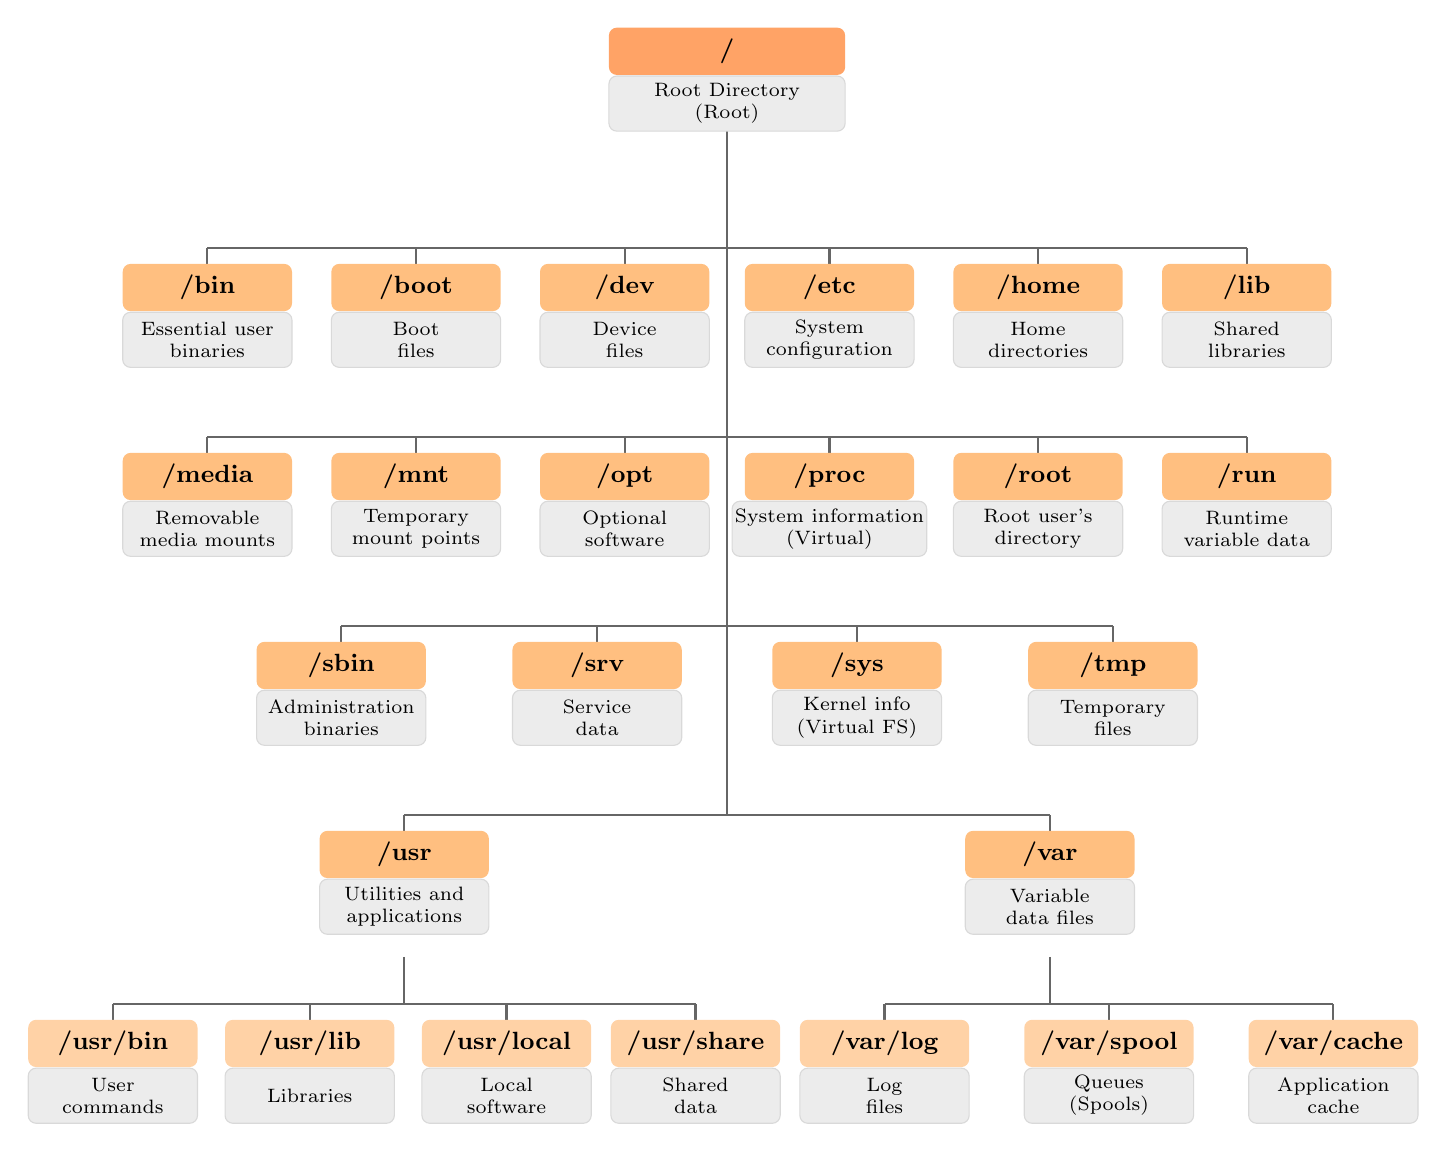
\begin{tikzpicture}[
    % Box styles (folders and descriptions)
    dir/.style={fill=#1, text=black, font=\bfseries\small, minimum width=2.15cm, minimum height=0.6cm, rounded corners=1mm, inner sep=0pt},
    desc/.style={fill=gray!15, draw=gray!30, text=black, font=\scriptsize, align=center, minimum width=2.15cm, minimum height=0.7cm, rounded corners=1mm, anchor=north, inner sep=1pt},
    treeline/.style={thick, draw=gray!80!black}
]

% ---------------------------------------------------------
% 1. TREE LINES (Connection structure)
% ---------------------------------------------------------
% Central trunk
\draw[treeline] (0, 0.5) -- (0, -8.2);

% Row 1 (Tier 1)
\draw[treeline] (-6.6, -1.0) -- (6.6, -1.0);
\foreach \x in {-6.6, -3.95, -1.3, 1.3, 3.95, 6.6} \draw[treeline] (\x, -1.0) -- (\x, -1.5);

% Row 2 (Tier 2)
\draw[treeline] (-6.6, -3.4) -- (6.6, -3.4);
\foreach \x in {-6.6, -3.95, -1.3, 1.3, 3.95, 6.6} \draw[treeline] (\x, -3.4) -- (\x, -3.9);

% Row 3 (Tier 3)
\draw[treeline] (-4.9, -5.8) -- (4.9, -5.8);
\foreach \x in {-4.9, -1.65, 1.65, 4.9} \draw[treeline] (\x, -5.8) -- (\x, -6.3);

% Row 4 (Tier 4) - usr and var
\draw[treeline] (-4.1, -8.2) -- (4.1, -8.2);
\foreach \x in {-4.1, 4.1} \draw[treeline] (\x, -8.2) -- (\x, -8.7);

% /usr subtree
\draw[treeline] (-4.1, -10.0) -- (-4.1, -10.6);
\draw[treeline] (-7.8, -10.6) -- (-0.4, -10.6);
\foreach \x in {-7.8, -5.3, -2.8, -0.4} \draw[treeline] (\x, -10.6) -- (\x, -11.1);

% /var subtree
\draw[treeline] (4.1, -10.0) -- (4.1, -10.6);
\draw[treeline] (2.0, -10.6) -- (7.7, -10.6);
\foreach \x in {2.0, 4.85, 7.7} \draw[treeline] (\x, -10.6) -- (\x, -11.1);


% ---------------------------------------------------------
% 2. BOXES AND TEXT (Nodes)
% ---------------------------------------------------------
% ROOT
\node[dir=orange!80!red!60, minimum width=3cm] (root) at (0, 1.5) {/};
\node[desc, minimum width=3cm] at (root.south) {Root Directory\\(Root)};

% --- FILA 1 ---
\node[dir=orange!50] (bin) at (-6.6, -1.5) {/bin};
\node[desc] at (bin.south) {Essential user\\binaries};

\node[dir=orange!50] (boot) at (-3.95, -1.5) {/boot};
\node[desc] at (boot.south) {Boot\\files};

\node[dir=orange!50] (dev) at (-1.3, -1.5) {/dev};
\node[desc] at (dev.south) {Device\\files};

\node[dir=orange!50] (etc) at (1.3, -1.5) {/etc};
\node[desc] at (etc.south) {System\\configuration};

\node[dir=orange!50] (home) at (3.95, -1.5) {/home};
\node[desc] at (home.south) {Home\\directories};

\node[dir=orange!50] (lib) at (6.6, -1.5) {/lib};
\node[desc] at (lib.south) {Shared\\libraries};

% --- FILA 2 ---
\node[dir=orange!50] (media) at (-6.6, -3.9) {/media};
\node[desc] at (media.south) {Removable\\media mounts};

\node[dir=orange!50] (mnt) at (-3.95, -3.9) {/mnt};
\node[desc] at (mnt.south) {Temporary\\mount points};

\node[dir=orange!50] (opt) at (-1.3, -3.9) {/opt};
\node[desc] at (opt.south) {Optional\\software};

\node[dir=orange!50] (proc) at (1.3, -3.9) {/proc};
\node[desc] at (proc.south) {System information\\(Virtual)};

\node[dir=orange!50] (rootdir) at (3.95, -3.9) {/root};
\node[desc] at (rootdir.south) {Root user's\\directory};

\node[dir=orange!50] (run) at (6.6, -3.9) {/run};
\node[desc] at (run.south) {Runtime\\variable data};

% --- FILA 3 ---
\node[dir=orange!50] (sbin) at (-4.9, -6.3) {/sbin};
\node[desc] at (sbin.south) {Administration\\binaries};

\node[dir=orange!50] (srv) at (-1.65, -6.3) {/srv};
\node[desc] at (srv.south) {Service\\data};

\node[dir=orange!50] (sys) at (1.65, -6.3) {/sys};
\node[desc] at (sys.south) {Kernel info\\(Virtual FS)};

\node[dir=orange!50] (tmp) at (4.9, -6.3) {/tmp};
\node[desc] at (tmp.south) {Temporary\\files};

% --- ROW 4 (Expansion parent nodes) ---
\node[dir=orange!50] (usr) at (-4.1, -8.7) {/usr};
\node[desc] at (usr.south) {Utilities and\\applications};

\node[dir=orange!50] (var) at (4.1, -8.7) {/var};
\node[desc] at (var.south) {Variable\\data files};

% --- ROW 5 (/usr children) ---
\node[dir=orange!35] (usrbin) at (-7.8, -11.1) {/usr/bin};
\node[desc] at (usrbin.south) {User\\commands};

\node[dir=orange!35] (usrlib) at (-5.3, -11.1) {/usr/lib};
\node[desc] at (usrlib.south) {Libraries};

\node[dir=orange!35] (usrlocal) at (-2.8, -11.1) {/usr/local};
\node[desc] at (usrlocal.south) {Local\\software};

\node[dir=orange!35] (usrshare) at (-0.4, -11.1) {/usr/share};
\node[desc] at (usrshare.south) {Shared\\data};

% --- ROW 5 (/var children) ---
\node[dir=orange!35] (varlog) at (2.0, -11.1) {/var/log};
\node[desc] at (varlog.south) {Log\\files};

\node[dir=orange!35] (varspool) at (4.85, -11.1) {/var/spool};
\node[desc] at (varspool.south) {Queues\\(Spools)};

\node[dir=orange!35] (varcache) at (7.7, -11.1) {/var/cache};
\node[desc] at (varcache.south) {Application\\cache};

\end{tikzpicture}
